\documentclass{article}

\usepackage[margin=1in]{geometry}
\usepackage{graphicx} 
\usepackage{gensymb}
\usepackage{amsmath}
\usepackage{multicol}
\usepackage[font=small,labelfont=bf]{caption}

\title{Introduction}

\begin{document}
\begin{center}
    {\huge{Introduction}}
\end{center}    
    
    Financial time series are beneficial for various purposes, for example to train machine learning models or to be used as inputs in market simulators. In these applications, the constraint of limited availability of large amounts of data can have an impact on the performance of the analysis. For these reasons, models, especially deep-learning ones, tend to overfit and struggle at generalizing. By augmenting a dataset we can contribute to the solution of this issue by providing a larger amount of data with respect to what is already accessible. Thanks to this result, companies can effectively  improve models and also use it to enhance strategy backtesting. 
    \subsection*{Characteristics of Time series}
    GANs can capture the temporal structures of financial time-series so as to generate the major stylized facts of price returns, including the linear unpredictability, the fat-tailed distribution, volatility clustering, the leverage effects, the coarse-fine volatility correlation, and the gain/loss asymmetry. 
    \begin{center}
        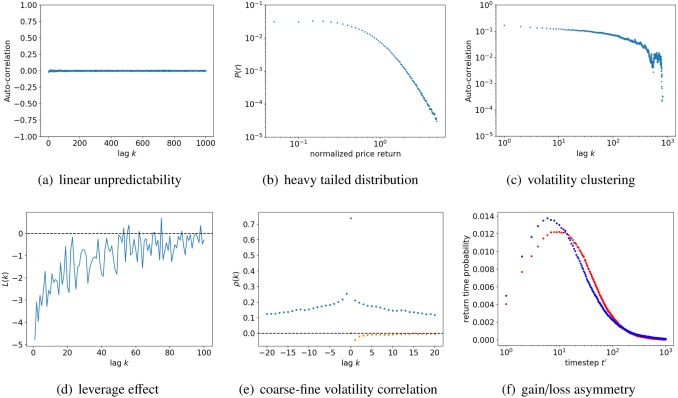
\includegraphics[scale = 0.7]{ts.jpeg}
    \end{center}
    In the studies of financial time-series, there are two major approaches, namely stochastic processes, and agent-based models, for modeling the financial time-series. However, it is difficult to recover all the major stylized facts with such explicit mathematical formulations. As an alternative approach, GANs have shown spectacular ability in the generation of data including realistic image, audio, natural language text, and financial data.\\
   
    \subsection*{General idea for the data}
    We began by taking a dataset of value stocks from the S&P 500 as we assumed it would have been easier to analyze financial series with more convenient intrinsic properties such as moderate volatility. In this way it was easier to interpret the results of our model since we could identify out of range peaks very easily. The reasoning behind was due to the fact that it is very hard to judge the performance of a model like this without a defined metric. As for now, we rely on our visual interpretation.\\ 
    
    \subsection*{Scalar method}
    Since the aim of the project is to augment a dataset to be used for further analysis in machine learning, we want to select the generated data that maintain the statistical properties mentioned above. For this reason we will apply a correction algorithm to correct the range of peaks of volatility. We could better observe the results thanks to the choice of our first dataset of stocks with low volatility. It was possible to capture the strange pattern of the series generated since some results did not mimic correctly  the normal behavior of certain types of stocks.\\ 
    
    \subsection*{Further implementation}
   We are now conducting more trials on different types of financial series starting from very volatile stocks. We would like to understand if the performance of the GAN is altered and then explore solutions on how to fix this, if this is the case.  In the future, our next step is to analyze the results of the series obtained with R, to analyze the statistical properties of the series. We would also like to develop a metric to evaluate accurately the performance of the model.
    
    
\end{document}
